\documentclass[DaoFP]{subfiles}
\begin{document}
\setcounter{chapter}{18}

\chapter{Kan Extensions}

If category theory keeps raising levels of abstraction it's because it's all about discovering patterns. Once patterns are discovered, it's time to study patterns formed by these patterns, and so on. 

We've seen the same recurring concepts described more and more tersely at higher and higher levels of abstraction. 

For instance, we first defined the product using a universal construction. Then we saw that the spans in the definition of the product were natural transformations. That led to the interpretation of the product as a limit. Then we saw that we can define it using adjunctions. We were able to combine it with the coproduct in one terse formula:
\[ (+) \dashv \Delta \dashv (\times) \]
Lao Tzu said: ``If you want to shrink something, you must first allow it to expand."

Kan extensions raise the level of abstraction even higher. Mac Lane said: ``All concepts are Kan extensions.''

\section{Closed Monoidal Categories}

We've seen how a function object can be defined as the right adjoint to the categorical product:
\[ \cat C (a \times b, c) \cong \cat C (a, [b, c]) \]
Here I used the alternative notation $[b, c]$ for the internal hom---the exponential $c^b$. 

An adjunction between two functors can be thought of as one being the pseudo-inverse of the other. They don't compose to identity, but their composition \emph{is} related to the identity functor through unit and counit. For instance, if you squint hard enough, the counit of the currying adjunction:
\[ \varepsilon_{b c} \colon [b, c] \times b \to c \]
suggests that $[b, c]$ embodies, in a sense, the inverse of multiplication. It plays a similar role as $c/b$ in:
\[ c/b \times b = c \]

In a typical categorical manner, we may ask the question: What if we replace the product with something else? The obvious thing, replacing it with a coproduct, doesn't work (thus we have no analog of subtraction). But maybe there are other well-behaved binary operations that have a right adjoint.

A natural setting for generalizing a product is a monoidal category with a tensor product $\otimes$ and a unit object $I$. If we have an adjunction:
\[ \cat C (a \otimes b, c) \cong \cat C (a, [b, c]) \]
we'll call the category \emph{closed monoidal}. In a typical categorical abuse of notation, unless it leads to confusion, we'll use the same symbol (a pair of square brackets)  for the monoidal internal hom as we did for the cartesian hom. There is an alternative \index{lollipop}lollipop notation for the right adjoint to the tensor product:
\[ \cat C (a \otimes b, c) \cong \cat C (a, b \multimap c) \]
It is often used in the context of \index{linear types}linear types.

The definition of the internal hom works well for a symmetric monoidal category. If the tensor product is not symmetric, the adjunction defines a \emph{left closed} monoidal category. The left internal hom is adjoint to the ``post-multiplication'' functor $(- \otimes b)$. The right-closed structure is defined as the right adjoint to the ``pre-multiplication'' functor $(b \otimes -)$. If both are defined than the category is called \index{bi-closed monoidal category}\emph{bi-closed}.


\subsection{Internal hom for Day convolution}

As an example, consider the symmetric monoidal structure in the category of co-presheaves with Day convolution:
\[ (F \star G) x = \int^{a, b} \cat C (a \otimes b, x) \times F a \times G b \]
We are looking for the adjunction:
\[ [\cat C, \Set] (F \star G, H) \cong  [\cat C, \Set] (F, [G, H]_{\text{Day}}) \]
The natural transformation on the left-hand side can be written as an end:
\[ \int_x \Set \big( \int^{a, b} \cat C (a \otimes b, x) \times F a \times G b, H x \big) \]
We can use co-continuity to pull out the coends:
\[ \int_{x, a, b} \Set \big( \cat C (a \otimes b, x) \times F a \times G b, H x \big) \]
We can then use the currying adjunction in $\Set$ (the square brackets stand for the internal hom in $\Set$):
\[ \int_{x, a, b} \Set \big( F a, [C (a \otimes b, x)  \times G b, H x] \big) \]
Finally, we use the continuity of the hom-set to move the two ends inside the hom-set:
\[ \int_{a} \Set \big( F a, \int_{x, b} [C (a \otimes b, x)  \times G b, H x] \big) \]
We get that the right adjoint to Day convolution is given by:
\[ \big([G, H]_{\text{Day}}\big) a = \int_{x, y} \big[\cat C(a \otimes x, y), [G x, H y]\big] \cong \int_x [G x, H (a \otimes x)]\]
The last transformation is the application of the Yoneda lemma in $\Set$.
\begin{exercise}
Implement the internal hom for Day convolution in Haskell. Hint: Use a type alias.
\end{exercise}

\subsection{Powering and co-powering}

In the category of sets, the internal hom (the function object, or the exponential) is isomorphic to the external hom (the set of morphisms between two objects):
\[ C^B \cong Set(B, C) \]
We can therefore rewrite the currying adjunction that defines the internal hom in $\Set$ as:
\[ \Set (A \times B, C)  \cong \Set \big(A, \Set (B, C)\big) \]
We can generalize this adjunction to the case where $B$ and $C$ are not sets but objects in some category $\cat C$. The external hom in any category is always a set. But the left-hand side is no longer a product. Instead it defines the action of a set $A$ on an object $b$:
\[ \cat C (A \cdot b, c) \cong \Set \big( A, \cat C (b, c)\big) \]
also known as the \emph{co-power}.

You may think of this action as adding together (taking a coproduct of) $A$ copies of $b$. For instance, if $A$ is a two-element set $\mathbf 2$, we get:
\[ \cat C (\mathbf 2 \cdot b, c) \cong \Set \big( \mathbf 2, \cat C (b, c)\big) \cong \cat C(b, c) \times \cat C(b, c) \cong \cat C(b + b, c) \]
In other words, 
\[ \mathbf 2 \cdot b \cong b + b \]
In this sense a co-power defines multiplication in terms of iterated addition, the way we learned it in school. 

If we multiply $b$ by the hom-set $\cat C (b, c)$ and take the coend over $b$'s, the result is isomorphic to $c$:
\[ \cat \int^b C(b, c) \cdot b \cong c \]
Indeed, the mappings to an arbitrary $x$ from both sides are isomorphic due to the Yoneda lemma:
\[ \cat C \big( \int^b \cat C(b, c) \cdot b, x\big) \cong \int_b \Set \big( \cat C(b, c), \cat C (b, x)\big) \cong \cat C (c, x)\]



As expected, in $\Set$, the co-power decays to the cartesian product.
\[ \Set (A \cdot B, C) \cong \Set \big( A, \Set(B, C)\big) \cong \Set (A \times B, C) \]

Similarly, we can express powering as iterated multiplication. We use the same right-hand side, but this time we use the mapping-in to define the \emph{power}:
\[ \cat C (b, A \pitchfork c) \cong \Set  \big(A, \cat C(b, c)\big) \]
You may think of the power as multiplying together $A$ copies of $c$. Indeed, replacing $A$ with $\mathbf 2$ results in:
\[ \cat C (b, \mathbf 2 \pitchfork c) \cong \Set  \big(\mathbf 2, \cat C(b, c)\big) \cong \cat C(b, c) \times \cat C(b, c) \cong \cat C (b, c \times c)\]
In other words:
\[ \mathbf 2 \pitchfork c \cong c \times c \]
which is a fancy way of writing $c^2$.

If we power $c$ by the hom-set $\cat C(c', c)$ and take the end over all $c$'s, the result is isomorphic to $c'$:
\[ \int_c \cat C (c', c) \pitchfork c \cong c' \]
This follows from the Yoneda lemma. Indeed the mappings from any $x$ to both sides are isomorphic:
\[ \cat C \big(x, \int_c \cat C (c', c) \pitchfork c\big) \cong \int_c \Set \big( \cat C(c', c), \cat C(x, c)\big)  \cong \cat C (x, c') \]


In $\Set$, the power decays to the exponential, which is the same as the hom-set:
\[ A \pitchfork C \cong C^A \cong \Set (A, C) \]
This is the consequence of the symmetry of the product.
\[ \Set(B, A \pitchfork C) \cong \Set (A, \Set(B, C)) \cong \Set (A \times B, C) \]
\[ \cong \Set (B \times A, C) \cong \Set (B, \Set (A, C))\]

\section{Inverting a functor}

One aspect of category theory is discarding information by performing lossy transformations; the other is recovering the lost information. We've seen examples of making up for lost data with free functors---the adjoints to forgetful functors. Kan extensions are another example. Both make up for data that is lost by a functor that is not invertible.

There are two reasons why a functor might not be invertible. One is that it may map multiple objects or arrows into a single object or arrow. In other words, it's not injective on objects or arrows. The other reason is that its image may not cover the whole target category. 

Consider for instance an adjunction $L \dashv R$. Suppose that $R$ is not injective, and it collapses two object $c$ and $c'$ into a single object $d$
\begin{align*}
R c &= d \\
R c' &= d
\end{align*}
$L$ has no chance of undoing it. It can't map $d$ to both $c$ and $c'$ at the same time. The best it can do is to map $d$ to a ``more general'' object $L d$ that has arrows to both $c$ and $c'$. These arrows are needed to define the components of the counit of the adjunction:
\begin{align*}
\varepsilon_c &\colon L d \to c
\\
\varepsilon_{c'} &\colon L d \to c'
\end{align*}
where $L d$ is both $L (R c)$ and $L (R c')$
\[
 \begin{tikzcd} [row sep=0.5cm, column sep=1cm]
 L d
 \arrow[d, "\varepsilon_c"]
 \arrow[dd, bend right, "\varepsilon_{c'}"']
 \\
 c
 \arrow[rr, red, dashed, ""]
 && d
 \arrow[ull, blue, bend right, dashed, "L"']
 \\
 c'
 \arrow[urr, red, dashed, "R"]
  \end{tikzcd}
\]


Moreover, if $R$ is not surjective on objects, the functor $L$ must somehow be defined on those objects of $\cat D$ that are not in the image of $R$. Again, naturality of the unit and counit will constrain possible choices, as long as there are arrows connecting these objects to the image of $R$. 

Obviously, all these constraints mean that an adjunction can only be defined in very special cases. Kan extensions are even weaker than adjunctions. 

If adjoint functors work like inverses, Kan extensions work like fractions. 

This is best seen if we redraw the diagrams defining the counit and the unit of an adjunction. In the first diagram, $L$ seems to play the role of $1/R$. In the second diagram $R$ pretends to be $1/L$.

\[
 \begin{tikzcd} [row sep=1cm, column sep=1cm]
 \cat C
 \arrow[rr, "\text{Id}", "" {name=ID, below} ]
 \arrow[d, bend right, "R"']
 && \cat C
 \\
 \cat D
  \arrow[urr, bend right, "L"']
 \arrow[Rightarrow, "\varepsilon",  to=ID]
 \end{tikzcd}
 \qquad
 \begin{tikzcd} [row sep=1cm, column sep=1cm]
 \cat D
 \arrow[rr, "\text{Id}", "" {name=ID, below} ]
 \arrow[d, bend right, "L"']
 && \cat D
 \\
 \cat C
  \arrow[urr, bend right, "R"']
 \arrow[Rightarrow, "\eta",  from=ID]
 \end{tikzcd}
\]

The right Kan extension $\text{Ran}_P F$ and the left Kan extension $\text{Lan}_P F$ generalize these by replacing the identity functor with some functor $F \colon \cat C \to \cat D$. The Kan extensions then play the role of fractions $F/P$. Conceptually, they undo the action of $P$ and follow it with the action of $F$.

\[
 \begin{tikzcd} [row sep=1cm, column sep=1cm]
 \cat C
 \arrow[rr, "F", "" {name=ID, below} ]
 \arrow[d, bend right, "P"']
 && \cat D
 \\
 \cat B
  \arrow[urr, bend right, "\text{Ran}_P F"']
 \arrow[Rightarrow, "\varepsilon",  to=ID]
 \end{tikzcd}
 \qquad
 \begin{tikzcd} [row sep=1cm, column sep=1cm]
 \cat C
 \arrow[rr, "F", "" {name=ID, below} ]
 \arrow[d, bend right, "P"']
 && \cat D
 \\
 \cat B
  \arrow[urr, bend right, "\text{Lan}_P F"']
 \arrow[Rightarrow, "\eta",  from=ID]
 \end{tikzcd}
\]

Just like with adjunctions, the ``undoing'' is not complete. The composition $\text{Ran}_P F \circ P$ doesn't reproduce $F$; instead it's related to it through the natural transformation $\varepsilon$ called the counit. Similiarly, the composition $\text{Lan}_P F \circ P$ is related to $F$ through the unit $\eta$.

Notice that the more information $F$ discards, the easier it is for Kan extensions to ``invert'' the functor $P$. In as sense, it only has to invert $P$ ``modulo $F$''.

Here's the intuition behind Kan extensions. We start with a functor $F$:
\[
 \begin{tikzcd} \cat C
 \arrow[r, "F"]
 & \cat D
  \end{tikzcd}
\]
There is a second functor $P$ that embeds $\cat C$ in another category $\cat B$. This embedding may be lossy and non-surjective. Our task is to \emph{extend} the definition of $F$ to the whole of $\cat B$. 

In the ideal world we would like the following diagram to commute:
\[
 \begin{tikzcd} \cat C
 \arrow[r, "F"]
 \arrow[d, "P"']
 & \cat D
 \\
 \cat B
\arrow[ur, "Kan_P F"']
  \end{tikzcd}
\]
But that would involve equality of functors, which is something we try to avoid at all cost. 

The next best thing would be to ask for a natural isomorphism between the two paths through this diagram. But even that seems like asking too much. So we finally settle down on demanding that one path be deformable into another, meaning there is a one-way natural transformation between them. The direction of this transformation distinguishes between right and left Kan extensions.

\section{Right Kan extension}

The right Kan extension is a functor $\text{Ran}_P F$ equipped with a natural transformation $\varepsilon$, called the counit of the Kan extension, defined as:
\[ \varepsilon \colon \text{Ran}_P F \circ P \to F\]
\[
 \begin{tikzcd} [row sep=1cm, column sep=1cm]
 \cat C
 \arrow[rr, "F", "" {name=ID, below} ]
 \arrow[d, bend right, "P"']
 && \cat D
 \\
 \cat B
  \arrow[urr, blue, bend right, "\text{Ran}_P F"']
 \arrow[Rightarrow, blue, "\varepsilon",  to=ID]
 \end{tikzcd}
\]

The pair $(\text{Ran}_P F, \varepsilon)$ is universal among such pairs $(G, \alpha)$, where $G$ is a functor $G \colon \cat B \to \cat D$ and $\alpha$ is a natural transformation:
\[ \alpha \colon G \circ P \to F \]
\[
 \begin{tikzcd} [row sep=1cm, column sep=1cm]
 \cat C
 \arrow[rr, "F", "" {name=ID, below} ]
 \arrow[d, bend right, "P"']
 && \cat D
 \\
 \cat B
  \arrow[urr, red, bend right, "G"']
 \arrow[Rightarrow, red, "\alpha",  to=ID]
 \end{tikzcd}
\]

Universality means that for any such $(G, \alpha)$ there is a unique natural transformation $\sigma \colon G \to \text{Ran}_P F$
\[
\begin{tikzcd}[row sep=2cm, column sep=2cm]
\cat C  \ar[d, "P"', "" {name=P}]
            \ar[r, "F", ""  {name=F, below, near start, bend right}]
&
\cat D
\\
\cat B
    \ar[ur, blue, bend left, "G", "" {name=G, below}]
    \ar[ur, blue, bend right, "\text{Ran}_P F"', "" {name=Ran}]
\arrow[Rightarrow, blue, "\sigma", from=G, to=Ran]
\end{tikzcd}
\]
 which factorizes $\alpha$, that is:
\[ \alpha = \varepsilon \cdot (\sigma \circ P) \]
Notice that this is a combination of vertical and horizontal compositions of natural transformations in which $\sigma \circ P$ is the whiskering of $\sigma$. Here's the same equation drawn in terms of string diagrams:

\[
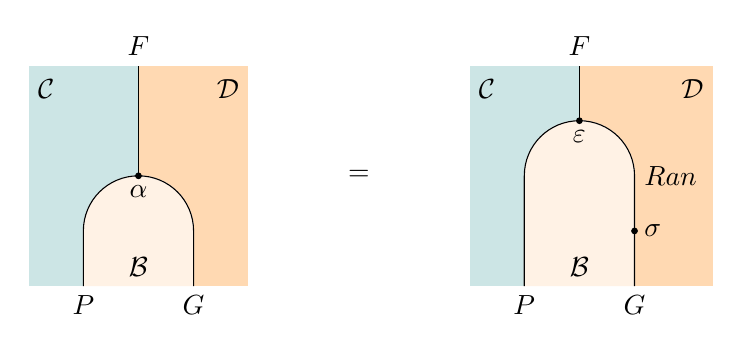
\begin{tikzpicture}
\def \dx {0.7}
\def \dy {0.7}

\def \xa{-3 * \dx};
\def \xb{-2 * \dx};
\def \xc{-1 * \dx};
\def \xd{0};
\def \xe{1 * \dx};

\def \ya{0};
\def \yb{1 * \dy};
\def \yc{2 * \dy};
\def \yd{3 * \dy};
\def \ye{4 * \dy};

% left background
\filldraw[fill=blue!50!green!20, draw=white] (\xa, \ye) rectangle (\xc, \ya);
% right background
\filldraw[fill=orange!30, draw=white] (\xc, \ye) rectangle (\xe, \ya);
% fill shape\yb
\path [fill=orange!10, draw=white]  (\xb, \ya) to (\xb, \yb) to [out=90, in=180]  (\xc, \yc) to  [out=0, in=90] (\xd, \yb) to (\xd, \ya);

% cup
\draw (\xb, \ya) to (\xb, \yb) to [out=90, in=180]  (\xc, \yc) to  [out=0, in=90] (\xd, \yb) to (\xd, \ya);
\draw (\xc, \yc) -- (\xc, \ye);

% natural transformations
\filldraw[black] (\xc, \yc) circle (1 pt);
\node [below] at (\xc, \yc) {$\alpha$};

% categories
\node[right] at (\xa, \ye - 0.3) {$\mathcal{C}$};
\node[left] at (\xe, \ye - 0.3) {$\mathcal{D}$};
\node[above] at (\xc, \ya) {$\mathcal{B}$};
% functors
\node [below] at (\xb, \ya) {$P$};
\node [below] at (\xd, \ya) {$G$};
\node [above] at (\xc, \ye) {$F$};

%-----------------
\node (eq) at (3 * \dx, \yc) {$=$};
% right diagram

\def \xa{5 * \dx};
\def \xb{6 * \dx};
\def \xc{7 * \dx};
\def \xd{8 * \dx};
\def \xe{9 * \dx + 0.3};

% left background
\filldraw[fill=blue!50!green!20, draw=white] (\xa, \ye) rectangle (\xc, \ya);
% right background
\filldraw[fill=orange!30, draw=white] (\xc, \ye) rectangle (\xe, \ya);
% fill shape
\path [fill=orange!10, draw=white]  (\xb, \ya) to (\xb, \yc) to [out=90, in=180]  (\xc, \yd) to  [out=0, in=90] (\xd, \yc) to (\xd, \ya);

% cup
\draw (\xb, \ya) to (\xb, \yc) to [out=90, in=180]  (\xc, \yd) to  [out=0, in=90] (\xd, \yc) to (\xd, \ya);
\draw (\xc, \yd) -- (\xc, \ye);

% natural transformations
\filldraw[black] (\xc, \yd) circle (1 pt);
\node [below] at (\xc, \yd) {$\varepsilon$};

\filldraw[black] (\xd, \yb) circle (1 pt);
\node [right] at (\xd, \yb) {$\sigma$};

% categories
\node[right] at (\xa, \ye - 0.3) {$\mathcal{C}$};
\node[left] at (\xe, \ye - 0.3) {$\mathcal{D}$};
\node[above] at (\xc, \ya) {$\mathcal{B}$};
% functors
\node [below] at (\xb, \ya) {$P$};
\node [below] at (\xd, \ya) {$G$};
\node [above] at (\xc, \ye) {$F$};
\node [right] at (\xd, \yc) {$\text{Ran}$};

\end{tikzpicture}
\]

As usual, a universal construction can be generalized to an adjunction---this time it's an adjunction between two functor categories:
\[ [\cat C, \cat D](G \circ P, F) \cong [\cat B, \cat D](G, \text{Ran}_P F) \]
For every $\alpha$ that is an element of the left-hand side, there is a unique $\sigma$ that is an element of the right-hand side.

In other words, the right Kan extension, if it exists for every $F$, is the right adjoint to functor pre-composition:
\[ (- \circ P) \dashv \text{Ran}_P \]
The component of the counit of this adjunction at $F$ is $\varepsilon$.

This is somewhat reminiscent of the currying adjunction:
\[ \cat C (a \times b, c) \cong \cat C (a, [b, c]) \]
in which the product is replaced by functor composition. (Of course, composition can be considered a tensor product only in the category of endofunctors.)

\subsection{Limits as Kan extensions}
 We have previously defined limits as universal cones. The definition of a cone involves two categories: the indexing category $\cat J$ that defines the shape of the diagram, and the target category $\cat C$. A diagram is a functor $D \colon \cat J \to \cat C$ that embeds the shape in the target category. 
 
 We can introduce a third category $\mathbf 1$: the terminal category that contains a single object and a single identity arrow. We can then use a functor $X$ from that category to pick the apex $x$ of the cone in $\cat C$. Since $\mathbf 1$ is terminal in $\mathbf{Cat}$, we also have the unique functor from $\cat J$ to it which, by the usual abuse of notation, we'll call $!$.
 
It turns out that the limit of $D$ is the right Kan extension of the diagram $D$ along $!$. First, let's observe that the composition $X \circ !$ maps the shape $\cat J$ to a single object $x$, so it does the job of the constant functor $\Delta_x$. It picks the apex of a cone. A cone with the apex $x$ is a natural transformation $\gamma$: 
\[
 \begin{tikzcd} [row sep=1cm, column sep=1cm]
 \cat J
 \arrow[rr, "D", "" {name=ID, below} ]
 \arrow[d, bend right, "!"']
 && \cat C
 \\
 \mathbf 1
  \arrow[urr, bend right, "X"']
 \arrow[Rightarrow, "\gamma",  to=ID]
 \end{tikzcd}
\]

The following diagrams illustrate this. On the left we have two categories: $\mathbf 1$ with a single object $*$, and $\cat J$ with three objects forming a shape for the diagram. On the right we have the image of $D$ and the image of $X \circ !$, which is the apex $x$. The three components of $\gamma$ connect the apex $x$ with the diagram. Naturality of $\gamma$ ensures that the triangles that form the sides of the cone commute.

\[
 \begin{tikzcd}
  & *
 \\
\\
1 
\arrow[rr, red]
\arrow[rd, red]
&& 2
\arrow[dl, red]
\\
& 3
 \end{tikzcd}
 \qquad
 \begin{tikzcd}
  & x
\arrow[ddr, "\gamma_2"]
 \arrow[ddl, "\gamma_1"']
 \arrow[ddd, "\gamma_3"]
 \\
\\
D 1 
\arrow[rr, red]
\arrow[rd, red]
&& D 2
\arrow[dl, red]
\\
& D 3
 \end{tikzcd}
 \]



The right Kan extension $(\text{Ran}_! D, \varepsilon)$ is the universal such cone. $\text{Ran}_! D$ is a functor from $\mathbf 1$ to $\cat C$, so it selects an object in $\cat C$. This is the apex $\text{Lim} D$ of the universal cone. 

Universality means that for any pair $(X, \gamma)$ there is a natural transformation $\sigma \colon X \to \text{Ran}_! D$ 
\[
\begin{tikzcd}[row sep=2cm, column sep=2cm]
\cat J  \ar[d, "!"', "" {name=P}]
            \ar[r, "D", ""  {name=F, below, near start, bend right}]
&
\cat C
\\
\mathbf 1
    \ar[ur, bend left, "X", "" {name=G, below}]
    \ar[ur, bend right, "\text{Ran}_! D"', "" {name=Ran}]
\arrow[Rightarrow, "\sigma", from=G, to=Ran]
\end{tikzcd}
\]
which factorizes $\gamma$. 

$\sigma$ has only one component $\sigma_*$, which is an arrow $h$ connecting the apex $x$ to the apex $\text{Lim} D$. The factorization:
 \[ \gamma = \varepsilon \cdot (\sigma \circ !) \]
reads, in components:
\[ \gamma_i = \varepsilon_i \circ h \]
It makes the triangles in the following diagram commute:
\[
 \begin{tikzcd}[row sep=1cm]
  & x
\arrow[dddl, "\gamma_1"']
\arrow[ddddr, "\gamma_3"]
\arrow[dddrr, "\gamma_2"]
\arrow[dd, dashed, "h"']
 \\
 \\
 & \text{Lim} D
\arrow[dl, blue, "\varepsilon_1"]
\arrow[ddr, blue, "\varepsilon_3"']
\arrow[drr, blue, "\varepsilon_2"]
\\
D 1 
\arrow[rrr, red]
\arrow[rrd, red]
&&& D 2
\arrow[dl, red]
\\
&& D 3
 \end{tikzcd}
 \]
This universal condition makes $\text{Lim} D$ the limit of the diagram $D$.


\subsection{Right Kan extension as an end}

Recall the ninja Yoneda lemma:
\[ F b \cong \int_{c} \mathbf{Set} (\mathcal{B}(b, c), F c) \]
Here, $F$ is a co-presheaf, that is a functor from $\cat B$ to $\Set$. The right Kan extensions of $F$ along $P$ generalizes this formula:
\[ (\text{Ran}_P F) b \cong \int_c \Set \big( \cat B (b, P c), F c\big) \]

This works for a co-presheaf. In general we are interested in $F \colon \cat C \to \cat D$, so we need to replace the hom-set in $\Set$ by a power. Thus he right Kan extension is given by the following end (if it exists):
 \[ (\text{Ran}_P F) b \cong \int_c \cat B (b, P c) \pitchfork F c \]
 
 The proof essentially writes itself: at every step there is only one thing to do. We start with the adjunction:
  \[ [\cat C, \cat D](G \circ P, F) \cong [\cat B, \cat D](G, \text{Ran}_P F) \]
and rewrite it using ends:
 \[ \int_c \cat D \big(G ( P c), F c\big) \cong \int_b \cat D\big(G b, (\text{Ran}_P F) b\big) \]
We substitute our formula to get:
 \[ \cong  \int_b \cat D\big(G b,\int_c \cat B (b, P c) \pitchfork F c \big)\]
We use the continuity of the hom-functor to pull the end to the front:
\[  \cong  \int_b \int_c \cat D\big(G b, \cat B (b, P c) \pitchfork F c \big) \]
Then we use the definition of power:
\[ \int_b \int_c \Set \big(  \cat B (b, P c), \cat D (G b, F c) \big) \]
and apply the Yoneda lemma:
\[ \int_c  \cat D \big(G (P c), F c\big) \]
This result is indeed the left-hand side of the adjunction.
 
If $F$ is a co-presheaf, the power in the formula for the right Kan extension decays to the exponential/hom-set:
  \[ (\text{Ran}_P F) b \cong \int_c \Set \big( \cat B (b, P c), F c\big) \]
This can be immediately translated to Haskell:
 \begin{haskell}
 newtype Ran p f b = Ran (forall c. (b -> p c) -> f c)
 \end{haskell}
 
 Notice also that, if $P$ has a left adjoint, let's call it $P^{-1}$, that is:
 \[ \cat B(b, P c) \cong \cat C(P^{-1} b, c) \]
 we could use the ninja Yoneda lemma to perform the end in:
 \[ (\text{Ran}_P F) b \cong \int_c \Set \big( \cat B (b, P c), F c\big) \cong \int_c \Set(\cat C(P^{-1} b, c), F c)\]
to get:
 \[  (\text{Ran}_P F) b \cong (F \circ P^{-1}) b \]
 Since the adjunction is a weakening of the idea of an inverse, this result is in agreement with the intuition that the Kan extension \emph{inverts} $P$ and follows it with $F$.
 
 \subsection{Left adjoint as a right Kan extension}
 
 We started by describing Kan extensions as a generalization of adjunctions. Looking at the pictures, if we have a pair of adjoint functors $L \dashv R$, we expect the left functor to be the right Kan extension of the identity along the right functor.
 \[ L \cong \text{Ran}_R \text{Id} \]
 
 Indeed, the counit of the Kan extension is the same as the counit of the adjunction:

 \[
 \begin{tikzcd} [row sep=1cm, column sep=1cm]
 \cat C
 \arrow[rr, "\text{Id}", "" {name=ID, below} ]
 \arrow[d, bend right, "R"']
 && \cat C
 \\
 \cat D
  \arrow[urr, bend right, "L"']
 \arrow[Rightarrow, "\varepsilon",  to=ID]
 \end{tikzcd}
\]
We also have to show universality:
\[
 \begin{tikzcd} [row sep=1cm, column sep=1cm]
 \cat C
 \arrow[rr, "\text{\text{Id}}", "" {name=ID, below} ]
 \arrow[d, bend right, "R"']
 && \cat C
 \\
 \cat D
  \arrow[urr, bend right, "G"']
 \arrow[Rightarrow, "\alpha",  to=ID]
 \end{tikzcd}
 \qquad %----%
\begin{tikzcd}[row sep=2cm, column sep=2cm]
\cat C  \ar[d, "R"', "" {name=P}]
            \ar[r, "R", ""  {name=F, below, near start, bend right}]
&
\cat D
\\
\cat D
    \ar[ur, bend left, "G", "" {name=G, below}]
    \ar[ur, bend right, "L"', "" {name=Ran}]
\arrow[Rightarrow, "\sigma", from=G, to=Ran]
\end{tikzcd}
\]
To do that, we have at our disposal the unit of the adjunction:
\[ \eta \colon \text{Id} \to R \circ L \]
We construct $\sigma$ as the composite:
\[ G \rightarrow G \circ \text{Id} \xrightarrow{G \circ \eta} G \circ R \circ L \xrightarrow{\alpha \circ L} \text{Id} \circ L \rightarrow L\]
In other words, we define $\sigma$ as:
\[ \sigma = (\alpha \circ L) \cdot (G \circ \eta) \]

We could ask the converse question: if $\text{Ran}_R \text{Id}$ exists, is it automatically the left adjoint to $R$? It turns out that we need one more condition for that: The Kan extension must be preserved by $R$, that is:

\[ R \circ \text{Ran}_R \text{Id} \cong \text{Ran}_R R \]
We'll see in the next section that the right-hand side of this condition defines the codensity monad.

\begin{exercise}
Show the factorization condition: 
\[ \alpha = \varepsilon \cdot (\sigma \circ R) \]
for the $\sigma$ that was defined above. Hint: draw the corresponding string diagrams and use the triangle identity for the adjunction.
\end{exercise}

 \subsection{Codensity monad}
 
 We've seen that every adjunction $L \dashv F$ produces a monad $F \circ L$. It turns out that this monad is the right Kan extension of $F$ along $F$. Interestingly, even if $F$ doesn't have a left adjoint, the Kan extension $\text{Ran}_F F$ is still a monad called the \emph{codensity monad} denoted by $T^F$:
 \[ T^F = \text{Ran}_F F \]
 
If we were serious about the interpretation of Kan extensions as fractions, a codensity monad would correspond to $F/F$. A functor for which this ``fraction'' is equal to identity is called codense.

To see that $T^F$ is a monad, we have to define monadic unit and multiplication:
\[ \eta \colon \text{Id} \to T^F \]
\[ \mu \colon T^F \circ T^F \to  T^F \]
 Both follow from universality. For every $(G, \alpha)$ we have a $\sigma$:
\[
 \begin{tikzcd} [row sep=1cm, column sep=1cm]
 \cat C
 \arrow[rr, "F", "" {name=ID, below} ]
 \arrow[d, bend right, "F"']
 && \cat D
 \\
 \cat D
  \arrow[urr, bend right, "G"']
 \arrow[Rightarrow, "\alpha",  to=ID]
 \end{tikzcd}
 \qquad
\begin{tikzcd}[row sep=2cm, column sep=2cm]
\cat C  \ar[d, "F"', "" {name=P}]
            \ar[r, "F", ""  {name=F, below, near start, bend right}]
&
\cat D
\\
\cat D
    \ar[ur, bend left, "G", "" {name=G, below}]
    \ar[ur, bend right, "T^F = \text{Ran}_F F"', "" {name=Ran}]
\arrow[Rightarrow, "\sigma", from=G, to=Ran]
\end{tikzcd}
\]

To get the unit, we replace $G$ with the identity functor $\text{Id}$ and $\alpha$ with the identity natural transformation. 

To get multiplication, we replace $G$ with $T^F \circ T^F$ and note that we have at our disposal the counit of the Kan extension:
\[ \varepsilon \colon  T^F \circ F \to F \]
We can define the corresponding $\alpha$:
\[ \alpha \colon T^F \circ T^F \circ F \to F \]
as the composite:
\[ T^F \circ T^F \circ F \xrightarrow{id \circ \varepsilon} T^F \circ F \xrightarrow{\varepsilon} F\]
or, using the whiskering notation:
\[ \alpha = \varepsilon \cdot (T^F \circ \varepsilon) \]
The corresponding $\sigma$ gives us the monadic multiplication.

Let's now show that, if we start from an adjunction:
\[ \cat C(L d, c) \cong \cat D (d, F c) \]
then $F \circ L$ gives us the codensity monad. Let's start with the mapping into $F \circ L$ from an arbitrary functor $G$:
\[ [\cat D, \cat D](G, F \circ L) \cong  \int_d \cat D (G d, F (L d)) \]
We can rewrite it using the Yoneda lemma:
\[ \cong \int_d \int_c \Set\big(\cat C(L d, c), \cat D (G d, F c)\big) \]
Here, taking the end over $c$ has the effect of replacing $c$ with $L d$. We can now use the adjunction:
\[ \cong \int_d \int_c \Set\big(\cat D(d, F c), \cat D (G d, F c)\big) \]
and perform the ninja-Yoneda integration over $d$:
\[ \cong \int_c \cat D (G (F c), F c) \]
This, in turn, defines a set of natural transformations:
\[ \cong [\cat C, \cat D](G \circ F, F) \]
The pre-composition by $F$ is the left adjoint to the right Kan extension:
\[ [\cat C, \cat D](G \circ F, F) \cong  [\cat D, \cat D] (G, \text{Ran}_F F)\]
This shows that $F \circ L$ is indeed the codensity monad for $F$.

Since every monad can be derived from some adjunction, it follows that every monad is a codensity monad for some adjunction.

Translating the codensity monad to Haskell, we get:
 \begin{haskell}
type Codensity f a = forall c. (a -> f c) -> f c
 \end{haskell}
This looks very similar to a continuation monad. In fact it turns into continuation monad if we choose \hask{f} to be the identity functor. We can think of \hask{Codensity} as taking a callback \hask{(a -> f c)} and calling it when the result of type \hask{a} becomes available. 

Here's the monad instance:
 \begin{haskell}
instance Monad (Codensity f) where
  return x = \k -> k x
  m >>= kl = \k -> m (\a -> (kl a) k)
 \end{haskell}
 Again, this is almost exactly like the continuation monad:
 \begin{haskell}
instance Monad (Cont r) where
  return x = Cont (\k -> k x)
  m >>= kl = Cont (\k -> runCont m (\a -> runCont (kl a) k))
\end{haskell}
This is why \hask{Codensity} has the performance advantages of the continuation passing style. Since it nests continuations ``inside out,'' it can be used to optimize long chains of binds that are produced by \hask{do} blocks. 

This property is especially important when working with free monads, which accumulate binds in tree-like structures. When we finally interpret a free monad, these accumulated binds require traversing the ever growing tree. For every bind, the traversal starts at the root. Compare this with the earlier example of reversing a list, which was optimized by accumulating functions in a FIFO queue. The codensity monad offers the same kind of performance improvement.

\section{Left Kan extension}

Just like the right Kan extension was defined as a right adjoint to functor pre-compositon, the left Kan extension is defined as the left adjoint to functor pre-composition:
\[ [\cat B, \cat D](\text{Lan}_P F , G) \cong  [\cat C, \cat D] (F, G \circ P) \]
 (There are also adjoints to \emph{post}-composition: they are called Kan lifts.)

Alternatively, $\text{Lan}_P F$ can be defined as a functor equipped with a natural transformation called the unit:
\[ \eta \colon F \to \text{Lan}_P F \circ P \]
\[
 \begin{tikzcd} [row sep=1cm, column sep=1cm]
 \cat C
 \arrow[rr, "F", "" {name=ID, below} ]
 \arrow[d, bend right, "P"']
 && \cat D
 \\
 \cat B
  \arrow[urr, bend right, "\text{Lan}_P F"']
 \arrow[Rightarrow, "\eta",  from=ID]
 \end{tikzcd}
\]
The pair $(\text{Lan}_P F, \eta)$ is universal, meaning that, for any other pair $(G, \alpha)$, where 
\[ \alpha \colon F \to G \circ P\] 
there is a unique mapping $\sigma \colon \text{Lan}_P F \to G$ 

\[
\begin{tikzcd}[row sep=2cm, column sep=2cm]
\cat C  \ar[d, "P"', "" {name=P}]
            \ar[r, "F", ""  {name=F, below, near start, bend right}]
&
\cat D
\\
\cat B
    \ar[ur, bend left, "G", "" {name=G, below}]
    \ar[ur, bend right, "\text{Lan}_P F"', "" {name=Lan}]
\arrow[Rightarrow, "\sigma", from=Lan, to=G]
\end{tikzcd}
\]
that factorizes $\alpha$:
\[ \alpha = (\sigma \circ P) \cdot \eta \]
or, using string diagrams:
\[
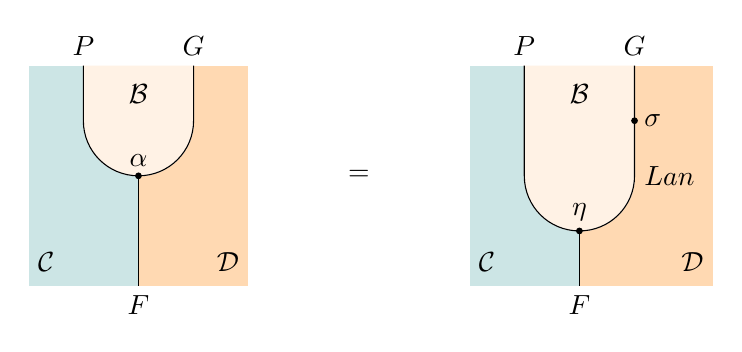
\begin{tikzpicture}
\def \dx {0.7}
\def \dy {-0.7}

\def \xa{-3 * \dx};
\def \xb{-2 * \dx};
\def \xc{-1 * \dx};
\def \xd{0};
\def \xe{1 * \dx};

\def \ya{0};
\def \yb{1 * \dy};
\def \yc{2 * \dy};
\def \yd{3 * \dy};
\def \ye{4 * \dy};

% left background
\filldraw[fill=blue!50!green!20, draw=white] (\xa, \ye) rectangle (\xc, \ya);
% right background
\filldraw[fill=orange!30, draw=white] (\xc, \ye) rectangle (\xe, \ya);
% fill shape\yb
\path [fill=orange!10, draw=white]  (\xb, \ya) to (\xb, \yb) to [out=270, in=180]  (\xc, \yc) to  [out=0, in=270] (\xd, \yb) to (\xd, \ya);

% cup
\draw (\xb, \ya) to (\xb, \yb) to [out=270, in=180]  (\xc, \yc) to  [out=0, in=270] (\xd, \yb) to (\xd, \ya);
\draw (\xc, \yc) -- (\xc, \ye);

% natural transformations
\filldraw[black] (\xc, \yc) circle (1 pt);
\node [above] at (\xc, \yc) {$\alpha$};

% categories
\node[right] at (\xa, \ye + 0.3) {$\mathcal{C}$};
\node[left] at (\xe, \ye + 0.3) {$\mathcal{D}$};
\node[above] at (\xc, \ya - 0.6) {$\mathcal{B}$};
% functors
\node [above] at (\xb, \ya) {$P$};
\node [above] at (\xd, \ya) {$G$};
\node [below] at (\xc, \ye) {$F$};

%-----------------
\node (eq) at (3 * \dx, \yc) {$=$};
% right diagram

\def \xa{5 * \dx};
\def \xb{6 * \dx};
\def \xc{7 * \dx};
\def \xd{8 * \dx};
\def \xe{9 * \dx + 0.3};

% left background
\filldraw[fill=blue!50!green!20, draw=white] (\xa, \ye) rectangle (\xc, \ya);
% right background
\filldraw[fill=orange!30, draw=white] (\xc, \ye) rectangle (\xe, \ya);
% fill shape
\path [fill=orange!10, draw=white]  (\xb, \ya) to (\xb, \yc) to [out=270, in=180]  (\xc, \yd) to  [out=0, in=270] (\xd, \yc) to (\xd, \ya);

% cup
\draw (\xb, \ya) to (\xb, \yc) to [out=270, in=180]  (\xc, \yd) to  [out=0, in=270] (\xd, \yc) to (\xd, \ya);
\draw (\xc, \yd) -- (\xc, \ye);

% natural transformations
\filldraw[black] (\xc, \yd) circle (1 pt);
\node [above] at (\xc, \yd) {$\eta$};

\filldraw[black] (\xd, \yb) circle (1 pt);
\node [right] at (\xd, \yb) {$\sigma$};

% categories
\node[right] at (\xa, \ye + 0.3) {$\mathcal{C}$};
\node[left] at (\xe, \ye + 0.3) {$\mathcal{D}$};
\node[above] at (\xc, \ya - 0.6) {$\mathcal{B}$};
% functors
\node [above] at (\xb, \ya) {$P$};
\node [above] at (\xd, \ya) {$G$};
\node [below] at (\xc, \ye) {$F$};
\node [right] at (\xd, \yc) {$\text{Lan}$};

\end{tikzpicture}
\]

This establishes one-to-one mapping between the sets of natural transformations. For every $\alpha$ on the left there is a unique $\sigma$ on the right:
\[  [\cat C, \cat D] (F, G \circ P) \cong [\cat B, \cat D](\text{Lan}_P F , G)  \]

\subsection{Colimits as Kan extensions}

Just like limits can be defined as right Kan extensions, colimits can be defined as left Kan extension. 

We start with an indexing category $\cat J$ that defines the shape of the colimit. The functor $D$ selects this shape in the target category $\cat C$. The apex of the cocone is selected by a functor from the terminal single-object category $\Cat 1$. The natural transformation defines a cocone from $D$ to $X$:
\[
 \begin{tikzcd} [row sep=1cm, column sep=1cm]
 \cat J
 \arrow[rr, "D", "" {name=ID, below} ]
 \arrow[d, bend right, "!"']
 && \cat C
 \\
 \Cat 1
  \arrow[urr, bend right, "X"']
 \arrow[Rightarrow, "\gamma",  from=ID]
 \end{tikzcd}
\]

Here's an illustrative example of a simple shape consisting of three objects and three morphisms (not counting identities). The object $x$ is the image of the single object $*$ under the functor $X$:
\[
 \begin{tikzcd}
1 
\arrow[rr, red]
\arrow[rd, red]
&& 2
\arrow[dl, red]
\\
& 3
\\
\\
& *
 \end{tikzcd}
 \qquad
 \begin{tikzcd}
D 1 
\arrow[rr, red]
\arrow[rd, red]
\arrow[dddr, "\gamma_1"']
&& D 2
\arrow[dl, red]
\arrow[dddl, "\gamma_2"]
\\
& D 3
\arrow[dd, "\gamma_3"]
\\
\\
&x
 \end{tikzcd}
 \]
The colimit is the universal cocone, which is given by the left Kan extension:
\[ \text{Colim}\; D = \text{Lan}_! D \]



\subsection{Left Kan extension as a coend}

Recall the ninja co-Yoneda lemma. For every co-presheaf $F$, we have:
\[ F b \cong \int^{c} \mathcal{B}(c, b) \times F c \]
The left Kan extension generalizes this formula:
\[ (\text{Lan}_P F)\, b \cong \int^{c} \cat B (P c, b) \times F c \]
For a general functor $F \colon \cat C \to \cat D$, we replace the product with the copower:
\[ (\text{Lan}_P F)\, b \cong \int^{c} \cat B(P c, b) \cdot F c \]

We prove this formula by considering a mapping out to some functor $G$. We represent the set of natural transformations as an end:
\[\int_b \cat D \big(\int^c \cat B(P c, b) \cdot F c, G b\big) \]
We pull out the coend, which turns into an end:
\[\int_b \int_c \cat D \big(\cat B(P c, b) \cdot F c, G b\big) \]
and plug in the definition of co-power:
\[\int_b \int_c \cat D \big(\cat B(P c, b), \cat D (F c, G b)\big) \]
We can now use the Yoneda lemma to integrate over $b$, replacing $b$ with $P c$:
\[\int_c \cat D (F c, G (P c))\big) \cong  [\cat C, \cat D] (F, G \circ P) \]
As long as the coend in question exists, it indeed gives us the left adjoint to functor pre-composition:
\[ [\cat B, \cat D](\text{Lan}_P F , G) \cong  [\cat C, \cat D] (F, G \circ P) \]

As expected, in $\Set$, the co-power decays to a cartesian product:
\[ (\text{Lan}_P F)\, b \cong \int^{c} \cat B (P c, b) \times F c \]

When translating this formula to Haskell, we replace the coend with the existential type. Symbolically:
 \begin{haskell}
 type Lan p f b = exists c. (p c -> b, f c)
 \end{haskell}
Currently, this is how we would encode the existential:
 \begin{haskell}
 data Lan p f e where
   Lan :: (p c -> b) -> f c -> Lan p f b
 \end{haskell}
 
 If the functor $P$ has a right adjoint, let's call it $P^{-1}$:
 \[ \cat B(P c , b) \cong \cat C(c, P^{-1} b) \]
 then we can use the ninja co-Yoneda lemma to get:
 \[  (\text{Lan}_P F)\, b \cong (F \circ P^{-1}) b \]
 thus reinforcing the intuition that a Kan extension inverts $P$ and follows it with $F$.
 
\subsection{Right adjoint as a left Kan extension}

We've seen that, when we have an adjunction $L \vdash R$, the left adjoint is related to the right Kan extension. Dually, if the right adjoint exists, it can be expressed as the left Kan extension of the identity functor:
\[ R \cong \text{Lan}_L \text{Id} \]
Conversely, if the left Kan extension of identity exists and it preserves the functor $L$:
\[ L \circ \text{Lan}_L \text{Id} \cong \text{Lan}_L L \]
than $\text{Lan}_L \text{Id}$ is the right adjoint of $L$. (Incidentally $\text{Lan}_F F$ is called the density comonad.)

The unit of Kan extension is the same as the unit of the adjunction:
\[
 \begin{tikzcd} [row sep=1cm, column sep=1cm]
 \cat D
 \arrow[rr, "\text{Id}", "" {name=ID, below} ]
 \arrow[d, bend right, "L"']
 && \cat D
 \\
 \cat C
  \arrow[urr, bend right, "R"']
 \arrow[Rightarrow, "\eta",  from=ID]
 \end{tikzcd}
\]
The proof of universality is analogous to the one for the right Kan extension.

\subsection{Day convolution as a Kan extension}

Day convolution is defined as a tensor product in the category of co-presheaves over a monoidal category $\cat C$:
\[ (F \star G) c = \int^{a, b} \cat C (a \otimes b, c) \times F a \times G b \]
Co-presheaves, that is functors in $[\cat C, \Set]$, can also be tensored using an \index{external tensor product}\emph{external tensor product}. An external product of two objects, instead of producing an object in the same category, picks an object in a different category. In our case, the product of two functors ends up in the category of co-presheaves on $\cat C \times \cat C$:
\[ \bar{\otimes} \colon [\cat C, \Set] \times [\cat C, \Set] \to [\cat C \times \cat C, \Set] \]
The product of two co-presheaves acting on a pair of objects in $\cat C \times \cat C$, is given by the formula:
\[ (F \bar{\otimes} G)\langle a, b \rangle = F a \times G b \]

It turns out that Day convolution of two functors can be expressed as a left Kan extension of their external product along the tensor product in $\cat C$:
\[ F \star G \cong \text{Lan}_{\otimes} (F \bar{ \otimes } G) \]
Pictorially:
\[
 \begin{tikzcd} [row sep=1cm, column sep=1cm]
 \cat C \times \cat C
 \arrow[rr, "F \bar{\otimes} G", "" {name=ID, below} ]
 \arrow[d, bend right, "\otimes"']
 && \Set
 \\
 \cat C
  \arrow[urr, bend right, "\text{Lan}_{\otimes} (F \bar{ \otimes } G)"']
 \end{tikzcd}
\]

Indeed, using the coend formula for the left Kan extension we get:
\[ (\text{Lan}_{\otimes} (F \bar{ \otimes } G)) c \cong \int^{\langle a, b\rangle} \cat C ( a \otimes b, c) \cdot (F \bar{ \otimes } G)\langle a, b\rangle\]

\[ \cong \int^{\langle a, b\rangle} \cat C ( a \otimes b, c) \cdot (F a \times G  b) \]
Since the two functors are $\Set$-valued, the co-power decays into the cartesian product:
\[ \cong \int^{\langle a, b\rangle} \cat C ( a \otimes b, c) \times F a \times G  b \]
and reproduces the formula for Day convolution.

\subsection{Kan extensions and optics}

Consider $\cat C^{op} \times \cat D$ an actegory with the action of a monoidal category $\cat M$. The full action is a functor:
\[ \bullet \colon \cat M^{op} \times \cat M \times \cat C^{op} \times \cat D \to  \cat C^{op} \times \cat D \]
\[  \langle m, n  \rangle \bullet \langle c, d \rangle = \langle m \bullet c, n \bullet d \rangle \]
Since we are going to take a coend over $m \colon \cat M$, we will use a shorthand for the diagonal part of this action:
\[ m \bullet \langle c, d \rangle = \langle m \bullet c, m \bullet d \rangle \]
With this notation, we can express the general optic in terms of the left Kan extension:
\[ \mathcal{O} \langle s, t \rangle \langle a, b \rangle \cong \left(\int^{m \colon \cat M} \text{Lan}_{m \bullet} \;\mathcal Y_{\langle a, b \rangle}\right) \langle s, t \rangle \]
where
\[ \mathcal Y_{\langle a, b \rangle} \langle c, d \rangle = (\cat C^{op} \times \cat D)(\langle a, b \rangle, \langle c, d \rangle) = \cat C(c, a) \times \cat D(b, d) \]
is the Yoneda functor.

Indeed, by definition, we have:
\[ \left( \int^m (\text{Lan}_{m \bullet} \; \mathcal Y_{\langle a, b \rangle} \right) \langle s, t \rangle \cong 
\int^{m, \langle c, d \rangle} \cat (\cat C^{op} \times \cat D)(m \bullet \langle c, d \rangle, \langle s, t \rangle) \cdot \mathcal Y_{\langle a, b \rangle} \langle c, d \rangle \]
We can now apply the co-Yoneda lemma to get:
\[ \cong \int^m \cat (\cat C^{op} \times \cat D)(m \bullet \langle a, b \rangle, \langle s, t \rangle)\]
which is the existential form of mixed optic.

The categories in question are depicted in this diagram:
\[
 \begin{tikzcd} [row sep=1cm, column sep=1cm]
 \cat C^{op} \times \cat D
 \arrow[rr, "\mathcal Y_{\langle a, b \rangle}", "" {name=ID, below} ]
 \arrow[d, bend right, "{\langle m, n \rangle \bullet}"']
 && \Set
 \\
 \cat C^{op} \times \cat D
  \arrow[urr, bend right, "{\text{Lan}_{\langle m, n \rangle \bullet}\; \mathcal Y_{\langle a, b \rangle}}"']
 \end{tikzcd}
\]

In general, with the Yoneda functor replaced by a general profunctor, the profunctor-functor:
\[ \Phi P = \int^m \text{Lan}_{m \bullet} \; P \]
is the Pastro-Street monad we used in deriving profunctor optics.

With this definition, we can derive the Pastro-Street comonad $\Theta$ as the right adjoint to $\Phi$. Let's use the notation $\text{Nat}$ for set of natural transformations in $[\cat C^{op} \times \cat D, \Set]$. We start with:
\[ \text{Nat}(\Phi P, Q) = \text{Nat}(\int^m \text{Lan}_{m \bullet} \;P, Q) \]
We pull out the coend using the co-continuity of the hom-functor:
\[\cong \int_m\text{Nat}( \text{Lan}_{m \bullet}\; P, Q) \]
 and use the adjunction that defines the left Kan extension:
\[ \cong \int_m\text{Nat}(P, Q \circ (m \bullet -)) \]
We use the continuity of the hom-functor to move the end in:
\[ \cong\text{Nat}(P,  \int_m Q \circ (m \bullet -)) \]
The result is:
\[ \text{Nat}(\Phi P, Q) \cong\text{Nat}(P,  \Theta Q) \]
where:
\[ (\Theta Q)\langle a, b \rangle = \int_m Q (m \bullet \langle a, b \rangle) \]


\section{Useful Formulas}
\begin{itemize}
\item Co-power:
\[ \cat C (A \cdot b, c) \cong \Set \big( A, \cat C (b, c)\big) \]
\item Power:
\[ \cat C (b, A \pitchfork c) \cong \Set  \big(A, \cat C(b, c)\big) \]
\item Right Kan extension:
\[ [\cat C, \cat D](G \circ P, F) \cong [\cat B, \cat D](G, \text{Ran}_P F) \]
 \[ (\text{Ran}_P F) e \cong \int_c \cat B (e, P c) \pitchfork F c \]
\item Right Kan extension in $\Set$:
  \[ (\text{Ran}_P F) e \cong \int_c \Set \big( \cat B (e, P c), F c\big) \]
\item Left Kan extension:
\[ [\cat B, \cat D](\text{Lan}_P F , G) \cong  [\cat C, \cat D] (F, G \circ P) \]
\[ (\text{Lan}_P F) e \cong \int^{c} \cat B(P c, e) \cdot F c \]
\item Left Kan extension in $\Set$:
\[ (\text{Lan}_P F) e \cong \int^{c} \cat B (P c, e) \times F c \]


\end{itemize}

\end{document}